\documentclass{exam}
\input{../preamble}
\pagestyle{headandfoot}
\firstpageheader{Physics}{Test on Unit 4: Forces}{}
\CorrectChoiceEmphasis{\color{red}\bfseries}
\SolutionEmphasis{\color{red}}


%\printanswers

\begin{document}
\begin{questions}

\question
What is the cause of an acceleration or a change in an object's motion?

\question
In the free-body diagram shown below, which of the following is the gravitational force acting on the balloon?

\begin{figure}[h!]
    \centering
    \includegraphics[width=4cm]{Figures/Balloon.png}
\end{figure}

\question
What is the tendency of an object to resists a change in motion?

\question
The statement by Newton that for every action there is an equal but opposite reaction is which of his laws of motion?

\question
The magnitude of the force of gravity acting on an object is \fillin\ .


\question
Friction is a force that always acts \fillin\ .

\question
Compared to its mass on Earth, the mass of a 10-kg object on the moon is \fillin\ .

\question
A tennis ball and a solid steel ball with the same diameter are dropped at the same time. In the absence of air resistance, which ball has the greater acceleration?

\question
A \SI{25}{N} falling object encounters \SI{6}{N} of air resistance. The magnitude of the net force on the object is \fillin\ .

\question
How much force is needed to accelerate a 8.0-kg physics book to an acceleration of \SI{3.0}{m/s^2}?

\question
A 20-N falling object encounters \SI{20}{N} of air resistance. The magnitude of the net force on the object is \fillin\ .

\question
An object's velocity vs time graph is shown below. During which interval is there no net force acting on the object?

\begin{figure}[h!]
    \centering
    \includegraphics[width=4cm]{Figures/Velocity.png}
\end{figure}

\question
A 35.0-N physics textbook rests on a table. What is the force the table exerts on the textbook?


\clearpage
\question
Which diagram below represents a box in equilibrium?

\begin{figure}[h!]
    \centering
    \includegraphics[width=5cm]{Figures/Equilibrium.png}
\end{figure}


\question
When forces acting on an object are balanced, which quantity of motion is zero?


\question
This graph shows weight versus mass for a group of objects on planet X. What is the acceleration due to gravity on planet X?

\begin{figure}[h!]
    \centering
    \includegraphics[width=4cm]{Figures/Weight.png}
\end{figure}

\question
What is the weight of a 7.5-kilogram object on the surface of Earth?

\question
Two forces, $F_1$ and $F_2$, are applied to a block on a frictionless, horizontal surface as shown below. If the magnitude of the block's acceleration is \SI{2.0}{m/s^2}, what is the mass of the block?

\begin{figure}[h!]
    \centering
    \includegraphics{Figures/Blocks.png}
\end{figure}

\question
The diagram represents forces acting on a block that accelerates \SI{5.0}{m/s^2} on a frictionless surface. What is the mass of the block?

\begin{figure}[h!]
    \centering
    \includegraphics{Figures/Motion.png}
\end{figure}

\question
A 56-kg object is given a net force of \SI{490}{N}. What is its acceleration?

\question
Which of the following is the cause of an acceleration or a change in an object's motion?

\question
In the free-body diagram, which is the magnitude of the gravitational force on the balloon?

\begin{figure}[h!]
\centering
\begin{tikzpicture}
\pgfplotsset{compat=1.11}
\def\s{6}
    \begin{axis}[
        width=10cm, height=7cm,
        axis line style={draw=none},
        ticks=none,
        axis lines=middle,
        ymin=-\s, ymax=\s,
        xmin=-\s, xmax=\s,
        clip=false,
    ]
    \fill (0,0) circle (3pt); %node[above=3pt]{\SI{12}{kg}};
    \draw[very thick,black,->] (0,0) -- (0,5.12) node[right] {\SI{5120}{N}};
    \draw[very thick,black,->] (0,0) -- (0.95,0) node[right] {\SI{950}{N}};   
    \draw[very thick,black,->] (0,0) -- (0,-4.05) node[left] {\SI{4050}{N}};
    \draw[very thick,black,->] (0,0) -- (-1.52,0) node[left] {\SI{1520}{N}}; 
    \end{axis}
\end{tikzpicture}
% \caption*{Figure: Free-body diagram of a hot-air balloon. Note: the vertical axis is not to scale with the horizontal one.}
\end{figure}

\question
Which of the following is the tendency of an object to remain at rest or to remain in motion?


\question
Newton said that an apple forcing its weight on a table will experience an upward force on it equal to its weight. This example expemplifies which of Newton's laws?

\question
What is weight?

\question
What is the contact force that acts in the direction opposite to the object's velocity?

% \question
% On Earth, acceleration due to gravity is $g=\SI{9.8}{m/s^2}$. On the Moon, however, acceleration due to gravity is weaker: $g_{\text{moon}} = \SI{1.6}{m/s^2}$. 

\question
A branch weighing \SI{20}{N} falls from the top of a tall tree and experiences \SI{4}{N} of air resistance. What is the magnitude of the net force on the branch?

\question 
The magnitude of the net force required to accelerate a \SI{4.0}{kg} physics book by \SI{2.0}{m/s^2} is \fillin[\SI{8.0}{N}] .

\question
Tweety, the canary who weights \SI{6}{N}, experiences \SI{6}{N} of air resistance as he launches off a branch. What is the net force on Tweety?

\question
A \SI{20}{N} physics book is at rest on a table. What is the magnitude of the force that the table exerts on the book?

\question
When all forces on an object are balanced, which quantity of motion is zero?

\question
What is the weight of a 2.00-kilogram cat?

\question
Two forces act upon a block. If the block's acceleration is \SI{2.0}{m/s^2}, what is mass of the block?

\begin{figure}[h!]
\centering
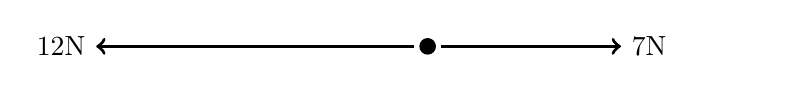
\begin{tikzpicture}
\pgfplotsset{compat=1.11}
\def\s{12}
    \begin{axis}[
        width=10cm, height=2cm,
        axis line style={draw=none},
        ticks=none,
        axis lines=middle,
        ymin=-\s, ymax=\s,
        xmin=-\s, xmax=\s,
        clip=false,
    ]
    \fill (0,0) circle (3pt); %node[above=3pt]{\SI{12}{kg}};
    \draw[very thick,black,->] (0.5,0) -- (7,0) node[right] {\SI{7}{N}};   
    \draw[very thick,black,->] (-0.5,0) -- (-12,0) node[left] {\SI{12}{N}}; 
    \end{axis}
\end{tikzpicture}
\end{figure}

\clearpage
\question
The free-body diagram below shows an object that is accelerating horizontally at \SI{6.0}{m/s^2}. What is the mass of the object?

\begin{figure}[h!]
\centering
\begin{tikzpicture}
\pgfplotsset{compat=1.11}
\def\s{20}
    \begin{axis}[
        width=8cm, height=5cm,
        axis line style={draw=none},
        ticks=none,
        axis lines=middle,
        ymin=-10, ymax=10,
        xmin=-\s, xmax=\s,
        clip=false,
    ]
    \fill (0,0) circle (3pt); %node[above=3pt]{\SI{12}{kg}};
    \draw[very thick,black,->] (1,0) -- (18,0) node[right] {\SI{18}{N}};   
    \draw[very thick,black,->] (-1,0) -- (-6,0) node[left] {\SI{6}{N}}; 
    \draw[very thick,black,->] (0,1) -- (0,10) node[right] {$F_{\text{N}}$}; 
    \draw[very thick,black,->] (0,-1) -- (0,-10) node[right] {$w$};
    \end{axis}
\end{tikzpicture}
\end{figure}

\question
A \SI{45}{kg} object is acted on by a net force of \SI{500}{N}. What is the object's acceleration?

\question
While building the pyramid of Giza, eight people accelerate a 2300-kg block of limestone to \SI{0.800}{m/s^2}, overcoming \SI{3000}{N} of friction. Assume each individual applies the same force. What is magnitude of the force applied by each person? (\textit{Hint}: Draw a free-body diagram.)

\begin{solution}
\vspace{1em}

\textbf{Known}: $a = \SI{0.800}{m/s^2}$, $m = \SI{2300}{kg}$, friction $f = \SI{3000}{N}$. 

\textbf{Unknown}: Individually applied force $F =$ ?

\vspace{1em}

By the vector sum in the free-body diagram,

\begin{equation*}
    F_{\mathrm{net}} = 8F - f\ ,
\end{equation*}

and by Newton's 2nd law (Eq.~4.4),

\begin{equation*}
    F_{\mathrm{net}} = m a = \SI{1840}{N}\ ,
\end{equation*}

implying that

\begin{equation*}
     8F - f = ma\ .
\end{equation*}

Solving for force,

\begin{equation*}
    F = \frac{ma + f}{8} = \SI{605}{N}\ .
\end{equation*}
\end{solution}
\vspace{1em}

\hrule

\begin{EnvUplevel}
\hspace{2cm}
\begin{minipage}{0.6\textwidth}
\textbf{Read the passage below. Then answer the following questions.}\\

Suppose a \SI{10000}{kg} rocket ship blasts off from a launching pad. The upward force is provided by the thrust ($F_{\text{T}}$) from its engines. See the free-body diagram to the right. Assume that the rocket moves only vertically (in a straight line) and that there is no air resistance or friction.
\end{minipage}%
\hspace{-2cm}
\begin{minipage}{0.5\textwidth}
\centering
    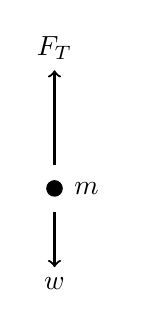
\begin{tikzpicture}
    \fill (0,0) circle[radius=3pt] node[right,inner sep=7pt] {$m$};
    \draw[->, thick] (0,0.3) -- (0,1.5)  node[above] {$F_{\text{T}}$};
    \draw[->, thick] (0,-0.3) -- (0,-1)  node[below] {$w$};
    \end{tikzpicture}
\end{minipage}

\end{EnvUplevel}

\question
Calculate the weight of the rocket.

\question
If the total thrust is \SI{130000}{N}, what is the net force on the rocket during blast-off?
(\textit{Hint}: Use the free-body diagram. In the vertical dimension, we may infer an \textit{up minus down rule})

\question
What is the rocket's vertical acceleration as it blasts off? Assume it moves vertically in one dimension.

\begin{solution}
\vspace{1em}

\textbf{Known}: $m = \SI{1.0e4}{kg}$, thrust $F_{\text{T}} = \SI{1.3e5}{N}$, $g = \SI{9.8}{m/s^2}$

\textbf{Unknown}: $a =$ ?

\begin{center}
    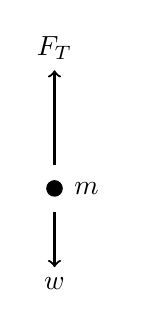
\begin{tikzpicture}
    \fill (0,0) circle[radius=3pt] node[right,inner sep=7pt] {$m$};
    \draw[->, thick] (0,0.3) -- (0,1.5)  node[above] {$F_{\text{T}}$};
    \draw[->, thick] (0,-0.3) -- (0,-1)  node[below] {$w$};
    \end{tikzpicture}
\end{center}

The weight of the rocket is 

\begin{equation*}
    w = m g = \SI{9.8e4}{N}
\end{equation*}

By the vector sum in the free-body diagram, net force is

\begin{equation*}
    F_{\mathrm{net}} = F_{\text{T}} - w = \SI{3.2e4}{N}
\end{equation*}

By Newton's 2nd Law, acceleration is

\begin{equation*}
   a = \frac{F_{\mathrm{net}}}{m} = \SI{3.2}{m/s^2}
\end{equation*}

\end{solution}

\question
The distance between two spheres of mass \SI{850}{kg} and \SI{970}{kg} is \SI{2.00}{m}. What is the gravitational force between the spheres?

\begin{solution}

\begin{equation*}
    F = \frac{G m M}{r^2} = \SI{1.38e-5}{N}
\end{equation*}
\end{solution}

\question 
What is the distance between the centers of mass for the objects below?
\vspace{-2em}

\begin{figure}[h!]
    \centering
    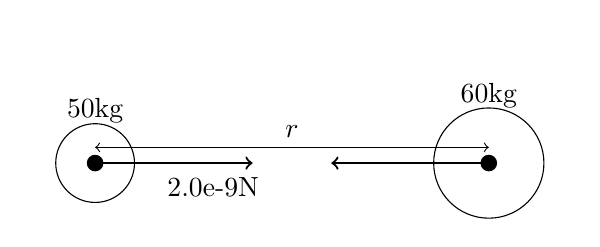
\begin{tikzpicture}
        \fill (0,0) circle[radius=3pt]; %node[below] {\tiny CM};
        \fill (5,0) circle[radius=3pt]; %node[below] {\tiny CM};
        \draw[<->] (0,0.2) -- (5,0.2);
        \node at (2.5,0.4) {$r$};
        \draw (0,0) circle (0.5cm) node[above,inner sep=0.5cm] {\SI{50}{kg}};
        \draw (5,0) circle (0.7cm) node[above,inner sep=0.7cm] {\SI{60}{kg}};
        \draw[->,thick] (0,0) -- (2,0);
        \draw[->,thick] (5,0) -- (3,0) ;
        \node at (1.5,-0.3) {\SI{2.0e-9}{N}};
        % \node at (3.8,-0.25) {$F$};
    \end{tikzpicture}
\end{figure}

\begin{solution}
Solving Newton's law of universal gravitation for distance leads to

\begin{equation*}
    r = \sqrt{\frac{GmM}{F}} = 
    \sqrt{\frac{\left(\SI{6.674e-11}{\frac{N \cdot m^2}{kg^2}}\right) \left(\SI{50}{kg}\right) \left(\SI{60}{kg}\right)}{\SI{2.0e-9}{N}}} = \SI{10.0}{m}
\end{equation*}
\end{solution}

\question 
The acceleration due to gravity on planetary bodies may be calculated using knowledge of mass and radius. For the parts below, use Eq.~(6.43) in your calculations and reference the NASA Planetary Fact Sheet (\href{https://nssdc.gsfc.nasa.gov/planetary/factsheet/}{link}).

\begin{parts}
\part What is the acceleration due to gravity on Earth?

\part What is the acceleration due to gravity on the Moon?

\begin{solution}

\begin{equation*}
    g = \frac{G M}{r^2} = \frac{(\SI{6.674e-11}{\frac{N \cdot m^2}{kg^2}})(\SI{7.3e22}{kg})}{(\SI{1.738e6}{m})^2} = \SI{1.6}{m/s^2}
\end{equation*}
\end{solution}

\part What is the acceleration due to gravity on Mars?

\begin{solution}

\begin{equation*}
    g = \frac{G M}{r^2} = \frac{(\SI{6.674e-11}{\frac{N \cdot m^2}{kg^2}})(\SI{6.42e23}{kg})}{(\SI{3.396e6}{m})^2} = \SI{3.71}{m/s^2} 
\end{equation*}
\end{solution}

% \part What is the acceleration due to gravity on the Sun?

\begin{solution}

\begin{equation*}
    g = \frac{G M}{r^2} = \frac{(\SI{6.674e-11}{\frac{N \cdot m^2}{kg^2}})(\SI{1.99e30}{kg})}{(\SI{6.96e8}{m})^2} = \SI{274}{m/s^2} 
\end{equation*}
\end{solution}
\end{parts}

\question
By what factor does the gravitational force between two objects change when the distance between them increases by a factor of 13?

\begin{solution}

\begin{equation*}
    \frac{F_{\text{new}}}{F_{\text{old}}} \sim \frac{G m M}{r^2} = \frac{(1)(1)(1)}{(13)^2} = \SI{5.9e-3}{} 
\end{equation*}
\end{solution}

\question
By what factor does the gravitational force between two objects change when the objects are brought $6 \times$ closer?

\begin{solution}

\begin{equation*}
    \frac{F_{\text{new}}}{F_{\text{old}}} \sim \frac{G m M}{r^2} = \frac{(1)(1)(1)}{\left(\frac{1}{6}\right)^2} = 6^2 = 36
\end{equation*}

The gravitational force gets 36 times stronger.
\end{solution}

\question
Let $F$ be the gravitational force between Earth and the Moon. If Earth was $10 \times$ more massive, the Moon was $4 \times$ more massive, and the distance between the bodies was $5 \times$ greater, by what factor would $F$ change? Does $F$ increase or decrease? 

\begin{solution}

\begin{equation*}
    \frac{F_{\text{new}}}{F} \sim \frac{G m M}{r^2} = \frac{(1)(10)(4)}{(5)^2} = \frac{40}{25} = 1.6
\end{equation*}

The gravitational force would increase by a factor of 1.6.
\end{solution}

\question
Consider a \SI{9.25}{lbs} baby sleeping in a crib. 

(Note: $\SI{1}{kg} = \SI{2.205}{lbs}$)

\begin{parts}
\part Calculate the gravitational force on the baby by the baby's \SI{135}{lbs} father, who stands \SI{30}{cm} away. 

\begin{solution} 
The separation distance is $r = \SI{30}{cm} = \SI{0.30}{m}$.
The masses of the baby and father are

\begin{equation*}
    m = \SI{9.25}{lbs} \times \frac{\SI{1}{kg}}{\SI{2.205}{lbs}} = \SI{4.20}{kg}
\end{equation*}
\vspace{-1em}

\begin{equation*}
    M = \SI{135}{lbs} \times \frac{\SI{1}{kg}}{\SI{2.205}{lbs}} = \SI{61.2}{kg}
\end{equation*}

\begin{equation*}
    F = \frac{G m M}{r^2} = \SI{1.9e-7}{N}
\end{equation*}
\end{solution}

\part Calculate the gravitational force on the baby by Jupiter, which is 390 million miles away.  

(Note: $\SI{1}{mi} \approx \SI{1609}{m}$)

\begin{solution} 
By the \textit{Planetary Fact Sheet} Jupiter's mass is $M = \SI{1.898e27}{kg}$. The distance between Jupiter and the baby is

\begin{equation*}
    r = \SI{390e6}{mi} \times \frac{\SI{1609}{m}}{\SI{1}{mi}} = \SI{6.28e11}{m}
\end{equation*}

The gravitational force by Jupiter is

\begin{equation*}
    F = \frac{G m M}{r^2} = \SI{1.3e-6}{N}
\end{equation*}
\end{solution}

% \part
% Calculate the gravitational force on the baby by the Sun.

% \begin{solution} 
% $M = \SI{1.989e30}{kg}$. The distance between the Earth and Sun is $r = \SI{1.496e11}{m}$.

% The gravitational force by the Sun is

% \begin{equation*}
%     F = \frac{G m M}{r^2} = \SI{2.49e-2}{N}
% \end{equation*}
% \end{solution}

% \part 
% Calculate the gravitational force on the baby by Earth. How does this force compare to the baby's weight, $w$?

% \begin{solution} 
% $M = \SI{5.9736e24}{kg}$, $r = R_{\mathrm{\Earth}} = \SI{6.376e6}{m}$.

% The gravitational force by Earth is

% \begin{equation*}
%     F = \frac{G m M}{r^2} = \SI{41.2}{N}
% \end{equation*}

% This force is exactly equal to the baby's weight, $w = mg$.
% \end{solution}

% \part
% Rank order the gravitational forces in the previous parts from least to greatest magnitude.


\part 
Compare the gravitational force from the father with the force from Jupiter. (Take their ratio.)

\begin{solution}
Jupiter exerts a gravitational force on the baby that is $7 \times$ greater than the force from the father.
\end{solution}
\end{parts}

\clearpage

\textbf{Instructions and Advice}
\begin{enumerate}
\setlength\itemsep{0.1ex}
    \item Show your work and answers on separate sheets of paper. Staple those sheets to this one. Although you don't need to staple extra scratch paper that you used for side calculations or brainstorming, your final product should be a detailed and organized solution of the problems.
    \item Start early. You'll probably have questions. Some problems are similar to those we cover in class. Review your class notes as you work on these problems.
    \item When in doubt, employ the GUESS method: Write the known quantities, the unknown, and equation(s) relating the known and unknown. Solve equations for the unknown. Substitute numbers at the \textit{end} of a problem.
    \item Use Desmos (available at \href{https://www.desmos.com/scientific}{https://www.desmos.com/scientific}).
    \item Don't give up on a problem without trying your best. Ask Mr.~Nunez and your peers for help.
    \item Keep in mind that future quizzes and tests are based in part on these problem sets. You should use these practice problems as a study guide.
    \item Write solutions that will make sense to \textit{you} one week from today.
    \item Practice makes you better. Re-visit these problems even after you solve them. Solving problems without looking at your notes will refine your problem-solving skills.
\end{enumerate}






\end{questions}
\end{document}